\chapter*{Appendix: Additional Functional Requirements\\ and Business Logic Model (2018)}
\label{appendix}

\vspace{-1cm}
\begin{center}
Eduard Hirsch and Paolo Dini
\end{center}

In order to see how to manage a more problematic use case based on reading historic data placed on the chain, delta debt as a additional requirement has been modelled. Therefore it should provide a showcase to forsee possible challenges for more complex tasks. The implementation details for the other requirements covered may be found in \cite{INTERLACE_D32}.

\section{Requirement: Debt Record Tracking}

Sardex gives credit to business network users based on their companies turn over as well as on their track record. Thus, the balance of an account, as described in the requirements of \cite{INTERLACE_D21} as well as \cite{INTERLACE_D31}, can go negative with any obligation to pay interest rates. However, that negative amount or debt needs to be paid back in 12 Month beginning from the transaction which puts the balance negative or increases the debt of an already negative balance.

To explain further, any transaction which increases the debt of an account, triggers a recording of that newly created debt-portion with a separately handled due date.

If an account receives a positive amount, then the "debt-portions" are paid back, starting from the oldest unpaid one.

\begin{figure}[htbp]
  \centering
  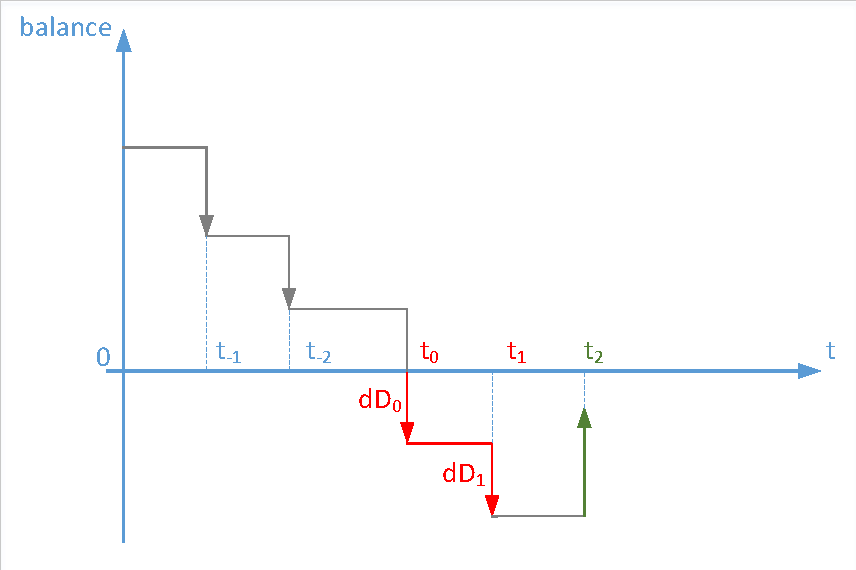
\includegraphics[width=0.5\textwidth, clip, trim=1mm 1mm 1mm 1mm]{Figures/deltadebt}
  \caption{\bf\small The delta debt progression}
  \label{fig:debt-graph}
\end{figure}

Figure \ref{fig:debt-graph} illustrates a transaction flow for a single account with 5 transactions and their timestamps named $t_i$, where $i$ covers the interval $[-2,2]$ in discrete steps of $1$. Two timestamps $t_j$ and $t_k$ having a $j>k$ imply that $t_j$ is older than $t_k$.

Let's assume a transaction as illustrated in the figure \ref{fig:debt-graph}, which turns a positive balance into a negative value. That event then defines a starting timestamp at $t_0$. This transaction at $t_0$ creates a debt of $balance$ reduced by the transaction $amount$ given that $balance >=0$ and $amount > balance$. Debt will be handled further as a positive value, thus, we define a debt at position $i$

\begin{asm}
	debt_{t_i} = \left\{\begin{array}{ll}
           |balance_{t_i} - amount_{t_i}| \+\+ & \IF i = 0 \AND balance_{t_0} >= 0 \AND amount > balance\\
           amount_{t_i} & \ELSEIF i >= 0 \AND balance_{t_i} < 0\\
           \UNDEF & \ELSE
        \end{array}\right .\-
\end{asm}

When declaring $TXID_i$ as the transaction id which is executed at time $t_i$ and $MBRID$ as the member id, we are defining a so called \textit{delta debt} as the following tuple

\begin{asm}
	dD_i = (t_i, TXID_i, Amount_{t_i}, DebtPos_{t_i}, MBRID)
\end{asm}

where the $Amount_{t_i}$ as well as $DebtPos_{t_i}$ are initialized with $debt_{t_i}$. In the following $Amount_{t_i}$ will always stay with its original value whereas $DebtPos_{t_i}$ will be reduced by an amount \textbf{received} by the same account.

The creation of a \textit{delta debt} can be described as following:

\begin{asm}
	\ASM{CreateDeltaDebt}(txid,currentDate,from,to,amount)=\+
		\LET balance = \ASM{balanceOf}(from)\+
			\IF (balance - amount) < 0 \THEN\+
				\LET debt =  \+\left\{\begin{array}{ll}
						|balance - amount|\+& \IF balance > 0\\
						amount & \ELSE
					\end{array}\right.\-\-
				\LET deltaDebt = (currentDate, txid, debt, debt, from)\+
					\ASM{WriteDeltaDebt}(deltaDebt)
\end{asm}

In order to pay back an open debt at every transfer it needs to be checked for possible debt clearances:

\begin{asm}
	\ASM{ClearDeltaDebt}(txid,credit,channel,from,to,amount)=\+
		\LET openDeltas = \ASM{SelectOpenDeltaDebtsFor}(to)\\
		\LET clearedAmount = amount\+
			\FORALL delta \IN openDeltas \DO\ \IF clearAmount > 0 \THEN\+
				\IF debtPos(delta) >= clearedAmount \THEN\+
					debtPos(delta) := debtPos(delta) - clearedAmount\\
					clearedAmount := 0\-
				\ELSE\+
					clearedAmount := clearedAmount - debtPos(delta)\\
					debtPos(delta) := 0\-\-
\end{asm}

Not working yet...
\begin{asm}
	\ASM{ClearDebt}(openDeltas, amount) =\+
		\CHOOSE delta \IN openDeltas  \WITH created(delta) = \ASM{SelectMinDelta}(openDelata) \DO\+
			\IF debtPos(delta) >= amount \THEN\+
				debtPos(delta) := debtPos(delta) - amount\-			
			\ELSE\+
				\LET clearedAmount = debtPos(delta)\+					
					\ASM{ClearDebt}(openDeltas, amount - clearedAmount)\\
					debtPos(delta) = 0
\end{asm}

In that ASM example we assume that $SelectOpenDeltaDebtFor$ is returning a list of open \textit{delta debt} entries which are sorted from the oldest to the newest as well as processed accordingly by the $forall$ loop.